\chapter{Proposed solution}
\label{chapter:proposedSolution}

\section{Approach definition}
\label{section:approachDefinition}

Now that we have analyzed the technical requirements and identified some of the challenges that could be encountered, we can continue with defining the solution for the described problem. Our approach would involve designing and developing a web application, keeping in mind its advantages over desktop applications, which we described in the previous section. The app would include two major parts: a web service developed in Java using the Spring Boot Framework and a client app built using the ReactJS Framework. The web sevice will define a REST API which will be used for communication between the client and the server. It will also handle the business logic and manage the persistence of data, which will be achieved by using a MySQL database. The client app will be the one that will run in the user's browser. As REST is stateless by definition, the client app will have to manage the session state. This will be achieved with the help of Redux - a predictable state containerfor JavaScript apps.

One important thing to keep in mind is that the application will be used for managing real documents of a public institution, which could potentially involve sensitive data. To secure our app, we will use features offered by Spring Security to enable JSON Web Token Authentication and manage access control.


\section{Technologies used}
\label{section:technologiesUsed}

In the following subsections of this chapter we will describe each of the chosen technologies in detail, with a strong focus on features that were decisive in choosing it over alternative technologies from the same branch.


\subsection{The Spring Framework}
\label{subsection:theSpringFramework}

The Spring Framework is an application framework for the Java platform which offers a wide range of features for modern Java-based applications. According to a survey from 2018, Spring is the most popular Web Framework worldwide in the JVM ecosystem (See Figure \ref{javaWebFrameworksTrendsImg}). It provides a large set of functionality and tools, making it suitable for a big variety of applications. In addition, its flexibility and focus on ease of use allow developers to focus on the application business logic rather than configurations and boilerplate code, thus increasing velocity, productivity and development speed.

\begin{figure}[H]
    \centering
    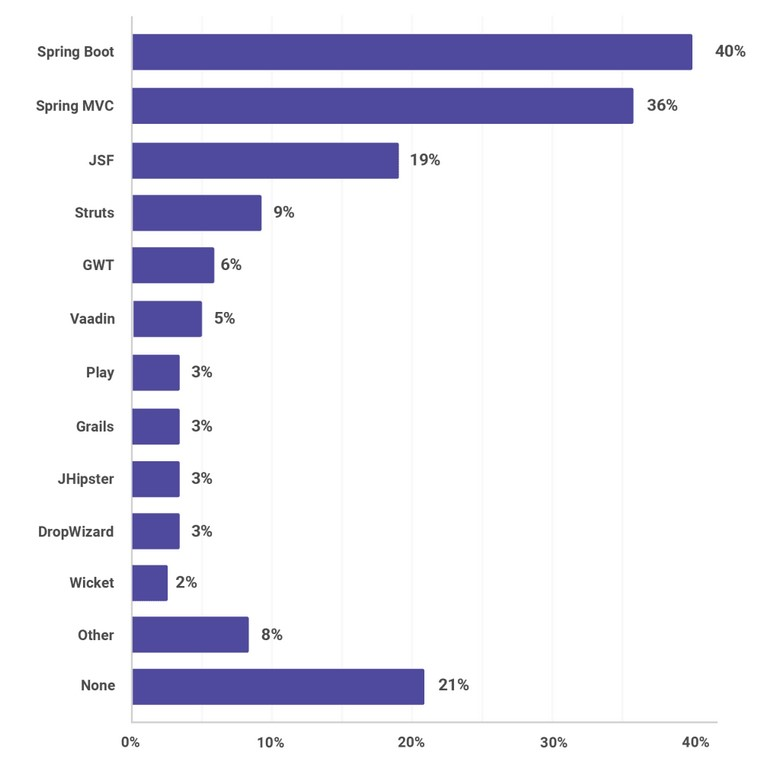
\includegraphics[width=4in]{images/javaWebFrameworksTrends}
    \caption{The most popular Java Web Frameworks according to the JVM Ecosystem report 2018 \cite{jvmEcosystemReport}}
    \label{javaWebFrameworksTrendsImg}
\end{figure}

One of the most important features offered by Spring is \textit{Inversion of Control} (IoC), achieved by \textit{Dependency Injection} (DI). According to this principle, objects are not responsible for creating their dependencies. Instead, they should be "injected" into the object through arguments passed to the constructor, setter methods or factory methods. In contrast to the classical way where each object is locating and instantiating all of its dependencies, the DI approach has several advantages. The most important one is achiving loose coupling, making it easier to interchange distinct implementations and maintain program modularity.

To achieve this, the Spring Framework uses an \textit{IoC container}. It is responsible for the instantiation, configuration and managing of the \textit{beans} - objects that will be used by the application (See Figure \ref{springIocContainer}). In order to know how each bean should be created and which dependencies injected, the IoC container needs additional configuration information. This is provided as metadata in form of XML, Java Configuration classes or Java annotations. In our project, we are going to use Java annotations as it is the most easy and straightforward way to configure beans.

\begin{figure}[H]
    \centering
    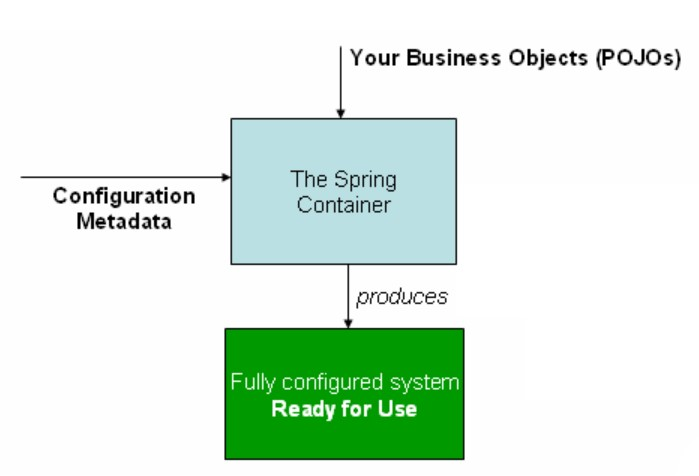
\includegraphics[width=4in]{images/springIocContainer}
    \caption{The Spring IoC Container \cite{springDocs}}
    \label{springIocContainer}
\end{figure}

Another advantage of Spring is that it uses well-known design patterns which are implemented under the hood:

\begin{itemize}
    \item All beans created by Spring are by default \textbf{Singletons}. This means that the IoC container creates only one instance for a bean and caches it so that it could then be used in multiple different places.
    \item Spring uses the \textbf{Factory Method Pattern} for bean creation. The \code{BeanFactory} class defines a list of \code{getBean()} methods, all of each are factory methods that could be used to create a bean with the the desired configuration. This functionality is extended by the \code{ApplicationContext} class, which adds the posibility of creating beans using external configurations like XML files or Java annotations.
    \item Spring uses the \textbf{Proxy Pattern} to control access to its beans. One tipical example where this is necessary is when using transactions. If we annotate a method as \code{@Transactional}, Spring guaranties its atomic execution and transactional consistency (hence the name). This is only possbile by intercepting the call through a proxy object that wraps our bean and would control the method execution.
    \item Spring uses the \textbf{Template Method Pattern} to minimize the amount of boilerplate code that is repeated again and again throughout projects. The \code{JdbcTemplate} class is a perfect example, providing an easy and intuitive way to execute database queries using predefined templates.
\end{itemize}


\subsection{Spring Boot}
\label{subsection:springBoot}

The Spring Framework provides a wide range of features for building enterprise and web applications, which makes it suitable for almost any type of use case. However, with the increasing amount of Spring features embedded into an application, the complexity of developing it also increases. Configurations grow in size and get diffucult to maintain.

Spring Boot was designed to solve exactly this problem. The module, while maintaining all of the power of its parent, significantly reduces the amount of configurations the developer has to make. It eliminates the need to write those parts of the code that always tend to be the same across multiple projects, like configuring a data source or a transaction manager. It also tends to simplify the deployment process, offering an embedded server which is ready to run as an alternative to manually setting up a deployment server.

All of this features result in an effortless and efficient development of web applications, which has made Spring Boot a widely popular choice for developing RESTful web services.


\subsection{Spring Security}
\label{subsection:proposedSolution}

\subsection{Spring JDBC}
\label{subsection:springJDBC}

\subsection{ReactJS Framework}
\label{section:reactJSFramework}

\subsection{Redux}
\label{section:redux}

\subsection{MySQL Database}
\label{section:mysqlDatabase}

% - performance (big amount of data)
% - relational vs non-relational db
% - where to store files? (db vs cloud)
% - db stuff (indexing / speeding up things ? highPerformanceMySQL)
% There's usually a lot of data, a moderate system will have over 1GB of data
% organized in tens of millions of records, so much data that managing it is a major part
% of the system. Older systems used indexed file structure such as IBM's VSAM and
% ISAM. Modern systems usually use databases, mostly relational databases. The
% design and feeding of these databases has turned into a sub-profession of its own.




% just so items from .bib would show up in bibliography
\cite{buildingRESTfulWebServicesWithSpring}
\cite{tamingTheStateInReact}
\cite{highPerformanceMySQL}


